\chapter{Fundamentals}
\label{cha:fundamentals}

This section describes the fundamental buildings blocks of the algorithm described in this thesis. It provides a quick overview and explanations of how the two different simulation techniques work. It does not describe in any way how the two different simulations might interact but instead describes them in total isolation.

\section{Rigid Body Simulations}
\label{sec:rigid_body_simulations}

Rigid bodies simulations is very similar to simple particle simulations. Simple particles are modeled as infinitesimal point masses, rigid bodies additional are defined by their dimension. This extension in space remains constant through out the whole simulation. A rigid body can therefore be thought of like a set of many particles. If a force is acting on any one of these point masses all the other connected masses in the rigid body are affected as well. Each point mass has a fixed mass $m_i$ and is located at fixed position $r_i$ inside the system. The total mass of the rigid body is then simply the sum of all the point masses combined
\[
M = \sum\limits_{i=1}^N m_i
\]

The position of the particles is defined relative to a local body coordinate system. The origin of coordinate system is the center of mass of the rigid body. The center of mass is calculated as 
\[
c = \frac{\sum m_i r_i}{M}
\]

In order to describe a rigid body simulation two variables are of central importance. First is the position \(x(t)\) of the rigid body in space. The second is the orientation \(q(t)\)in space. Both these variables are defined in relation to the world coordinate system. The quaternion \(q(t)\) is used to represent the rotation, as quaternions offer a number of practical advantages over rotation matrices during the simulation.
\begin{figure}[htbp]
\centering
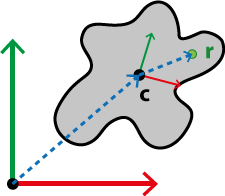
\includegraphics[scale=0.55]{images/rigid_body_1.png}
\caption{Rigid body model illustration}
\label{img:rigid_body}
\end{figure}
By definition only the affine transformations of rotation and translation can apply to any rigid body. The main task of the rigid body simulation is therefore to calculate these to variables over time \(t\).

The physics behind the rigid body simulation is based on Newton's laws of motion. Most importantly the first law stating that if no force is acting on an object, the velocity of the object will remain constant. Thus follows that the simulation has to model all forces acting on the body. These forces are the only causes for a change in the bodies state and thus its position and orientation in space.

\begin{itemize}
\item Two parts of force, Linear and Angular
\item Formulas for Linear and Angular forces
\item Integrating velocities over time
\item Using impulses to directly model velocities
\item Overview rigid body minimal state variables
\item Simple simulation loop
\end{itemize}

\section{Shape Matching}
\label{sec:shape_matching}

Shape Matching is an geometrically motivated approach to simulating deformable objects. It describes objects as a collection of points and does not need connectivity informations. By trading in physical correctness the technique is able to provide an unconditionally stable simulation. 

The main concept of this deformable model is to replace the system of forces and energies between the different particles by simple geometric constraints and distances. All points are moved to goal positions which are obtained by shape matching the original rest state of the object to the currently deformed state of the object. These well-defined goal positions are computationally easy to obtain and provide an unconditionally stable simulation.

\begin{figure}[h]
\centering
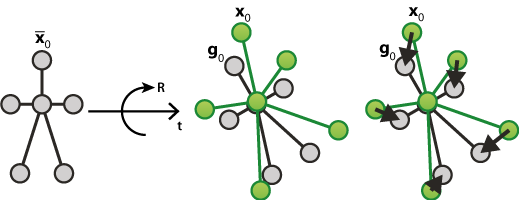
\includegraphics[scale=0.75]{images/shape_matching.png}
\caption{Shape matching illustration}
\label{img:shape_matching}
\end{figure}

The algorithm only takes a set of particles and there initial configuration as inputs. Each particle has four variables
\begin{align*}
m_i &, \text{the mass} \\
\bar{x}_i &, \text{the rest position} \\
x_i &, \text{the current position} \\
v_i &, \text{the velocity}
\end{align*}
The integration scheme uses the goal positions \(g_i\) to move the particles to the desired goal positions. The amount of movement can be directly modeled as a simple stiffness parameter \(\alpha\). A stiffness parameter if \(1\) thus basically doesn't allow for any deformation as the particles are always moved to their ideal transformed state. By using all these information and the external forces (i.e. gravity) the integration step becomes:

\begin{align}
v_i(t+h) &= v_i(t) + \alpha * \frac{g_i(t)-x_i(t)}{h} + h * f_{ext}(t)/m_i \\
x_i(t=h) &= x_i(t) + h * v_i(t+h)
\end{align}

The goal position \(g_i\) is obtained by shape matching the rest shape to the current deformed shape. The problem shape matching solves is thus defined by finding the rotation matrix \(R\) and the translation vector \(t\) between the two sets of points \(\bar{x}_i\) and \(x_i\). The desired matrix \(R\) and vector \(t\) minimize the following term:

\begin{equation}
\sum\limits_i m_i(R(\bar{x}_i-\bar{t})+t-x_i)^2
\label{eq:minimize_shape_matching}
\end{equation}

The optimal translation vectors are simply the respective center of masses of the rest shape and the deformed shape.

\begin{equation}
\bar{t} = \bar{c} = \frac{\sum_{i} m_i \bar{x}_i}{\sum_{i}m_i}, t = c = \frac{\sum_{i} m_i x_i}{\sum_{i}m_i}
\end{equation}

Unfortunately the optimal rotation matrix is not as simple to compute. The equation \ref{eq:eq:minimize_shape_matching} has to be simplified. The first step is to define relative positions for all points with respect to their center of mass.

\begin{gather}
q_i = \bar{x}_i - \bar{c}, p_i = x_i - c \\
\sum\limits_i m_i(Rq_i-p_i)^2
\end{gather}

The next insight is to actually find the optimal linear transformation \(A\) instead of the optimal rotation matrix \(R\).  Calculating the derivative with respect to all coefficients of \(A\) and setting it to zero gives the optimal linear transformation.

\begin{equation}
A = (\sum_i m_i p_i q_i^\top)(\sum_i m_i q_i q_i^\top)^{-1}=A_{pq}A_{qq}
\end{equation}

\(A_{qq}\) is a symmetric matrix can therefore contains no rotational part. All the rotation is encapsulated in \(A_{pp}\). The optimal rotation matrix can now be found by calculating the polar decomposition \(A = RS\). This allows to finally write down the goal position for each particle as

\begin{equation}
g_i = R(\bar{x}_i - \bar{c}) + c
\end{equation}

\section{Position Based Dynamics}
\label{sec:position_based_dynamics}

Position based dynamics is a method which omits the traditional force based approach simulate dynamics systems but instead directly works on the positions to simulate deformable objects. This means it also is not physically correct but instead provides an efficient unconditionally stable simulation. Like shape matching it also tries to satisfy constraints in order to arrive at stable end positions. But instead of one global constraint, the shape, position based dynamics handles many different constraints. These constraints either model the physical properties of the object and are thus fixed throughout the simulation, or are generated on demand in the case of collision constraints used to resolve collisions. Also as the name implies position based dynamics only works with the position of the particles updating them directly. The velocity of the particle is solely determined by the difference in positions overtime. This is best illustrated by the the pseudocode of the simulation loop.

\begin{algorithm}[h!]
\caption{Position based dynamics simuation}
\begin{algorithmic}[1]
\FORALL{vertices $i$}
	\STATE{initalize $x_i=\bar{x}_i, v_i =\bar{v}_i, w_i = 1/m_i$}
\ENDFOR
\LOOP
	\FORALL{vertices $i$} \STATE{$v_i \gets v_i + \Delta t w_i f_{ext}(x_i)$}\ENDFOR
	\STATE{dampVelocities($v_1,...,v_N$)}
	\FORALL{vertices $i$} \STATE{$p_i \gets x_i + \Delta t v_i$}\ENDFOR
	\FORALL{vertices $i$} \STATE{generateCollisionConstraints$(x_i\rightarrow p_i)$} \ENDFOR
	\WHILE{$i \leq solverIterations$}
		\STATE{projectConstraints$(C_1,...,C_{M+M_{coll}},p_1,...,p_N)$}
	\ENDWHILE
	\FORALL{vertices $i$} 
		\STATE{$v_i \gets (p_i-x_i)/\Delta t$}
		\STATE{$x_i \gets p_i$}
	\ENDFOR
	\STATE{velocityUpdate$(v_1,...,v_N)$}
\ENDLOOP
\end{algorithmic}
\end{algorithm}

The first key insight into the algorithm occurs in lines 9-11. Here positions for all vertices are estimated using the current velocity and the time step. This step is completely unrestricted and just predicts and estimates a position which is then later redefined. Line 15-17 illustrate this refinement. A Gauss-Seidel type iteration is used to satisfy all constraints defined for the system. These constraints mostly model the inherent structure of object currently simulated but another important aspect handled here are collisions with are just another constraint for the system and generated in each time step after estimating the position. The idea is to iterate over all constraints multiple times so that the particles are projected to valid locations with respect to the given constraint. The final vital piece of the algorithm can be seen in lines 18-21. After all constraints have been satisfied as best as possible the estimated positions alone are used to update the state of all vertices. The velocity of the particle is solely calculated by the difference of the new estimated position and the former position. This integration scheme is unconditionally stable as it doesn't just extrapolate into the future like traditional explicit schemes do. Instead it uses the physically valid positions computed with the constraint solver.

\section{Oriented Particles}
\label{sec:oriented_particles}

\begin{itemize}
\item Oriented particles combine shape matching and position based dynamics approach
\item Improves upon Shape Matching especially in areas of low density
\item Shape Matching is extend with orientation information for each particle
\item Enables simulation of extremely sparse regions with fewer particles
\item Describing moment matrix for body
\item Derive moment matrix for combination of multiple particles
\item Derive moment matrix for single particle
\item Instead of using the goal positions to get velocities, PBD approach of calculating velocities from difference between new position and old position
\item Description of the initial prediction step for both position and orientation
\item Description of shape matching constraints and implicit shape matching
\item Resolving collisions between particle and plane
\item Resolving collisions between particle and particle
\item Using Gauss Seidel type iterations to satisfy all shape matching constraints
\item Updating the current state using integration scheme
\item Handling friction friction in PBD
\end{itemize}
